\documentclass[10pt]{article}
\usepackage[margin=0.9in]{geometry}
\usepackage{amsmath,amssymb,mathtools}
\usepackage{graphicx}
\usepackage{hyperref}
\setlength{\parskip}{4pt}
\setlength{\parindent}{0pt}

\begin{document}
\begin{center}
{\Large FRC 100.006 — Born Rule from Resonant Equilibrium (Deterministic Derivation)}\\
{\large October 2025}\\[4pt]
H. Servat
\\[4pt]
\small DOI: \href{https://doi.org/10.5281/zenodo.17438360}{10.5281/zenodo.17438360}
\\[4pt]
\small DOI: \href{https://doi.org/10.5281/zenodo.17438360}{10.5281/zenodo.17438360}
\end{center}

\section*{Abstract}
We present a deterministic derivation of the Born rule within Fractal Resonance Cognition (FRC). Collapse is modeled as resonance phase--locking to pointer attractors; probabilities emerge from a resonant equilibrium of microstates. With an explicit coherence functional and a small drift, the stationary measure yields $p_j\!\propto\!|\alpha_j|^2$ under broad conditions. We include toy simulations that converge to Born weights and list concrete falsification tests.

\section*{1. Motivation}
Deterministic collapse (FRC 100.003) and its thermodynamic legitimacy (100.005) demand a clean account of probability. We assume a distribution of microstates (hidden phases) that flows under a small coherence drift and show that the stationary distribution in measurement contexts is proportional to squared amplitudes.

\section*{2. Setup}
Write an initial state $|\psi\rangle=\sum_j \alpha_j |a_j\rangle$ in the pointer basis $\{|a_j\rangle\}$. Let $\mu(\phi)$ denote microstates (phases/latent variables) with density $\rho(\phi,0)$, and define a simplicity prior that penalizes phase dispersion.

\paragraph{Coherence functional (explicit).}
To make the drift fully concrete we use a von~Mises--type coherence gauge that rewards phase alignment with sector phases $\{\phi_j\}$:
\begin{equation}
 C(\phi;\alpha) \;=\; \sum_{j} |\alpha_j|^2\, e^{\beta\cos(\phi-\phi_j)} ,\qquad \beta>0.\label{eq:Cdef}
\end{equation}
Other choices are possible; \eqref{eq:Cdef} suffices for the toy dynamics below and makes the drift reproducible. Under a weak coherence drift the continuity equation in microstate space reads
\begin{equation}
 \partial_t \rho \;=\; -\nabla\!\cdot (\rho\,\mathbf{v})\; ,\qquad \mathbf{v} \;\propto\; \nabla_{\phi} \ln C(\phi;\alpha).\label{eq:continuity}
\end{equation}

\section*{3. Equilibrium and weights}
At stationarity ($\partial_t\rho=0$ in Eq.~\eqref{eq:continuity}) a detailed--balance analogue yields
\begin{equation}
 \rho_\star(\phi)\;\propto\; \exp\big[-\mathcal{F}(\phi;\alpha)/k_*\big],\label{eq:rhostar}
\end{equation}
with an effective potential $\mathcal{F}$ minimized when microstates align with pointer phases. \textit{Dimensional comment:} the constant $k_*$ sets the coherence--entropy scaling (as in FRC~100.005/566.001) so that $\mathcal{F}/k_*$ is dimensionless. Integrating $\rho_\star$ over the attraction basin of sector $j$ gives a sector weight $p_j\!\propto\!|\alpha_j|^2$ under broad regularity assumptions; see Appendix~A. The result is robust to small perturbations in the drift and prior.

\section*{4. Simulations (toy, reproducible)}
We implement two toys (\verb|code/100.006/make_figures.py|): (i) sampling microstates and evolving them with a coherence drift; (ii) a direct equilibrium sampler with an $|\alpha|^2$ bias. Figures show convergence of empirical sector frequencies to $|\alpha_j|^2$.

\begin{center}
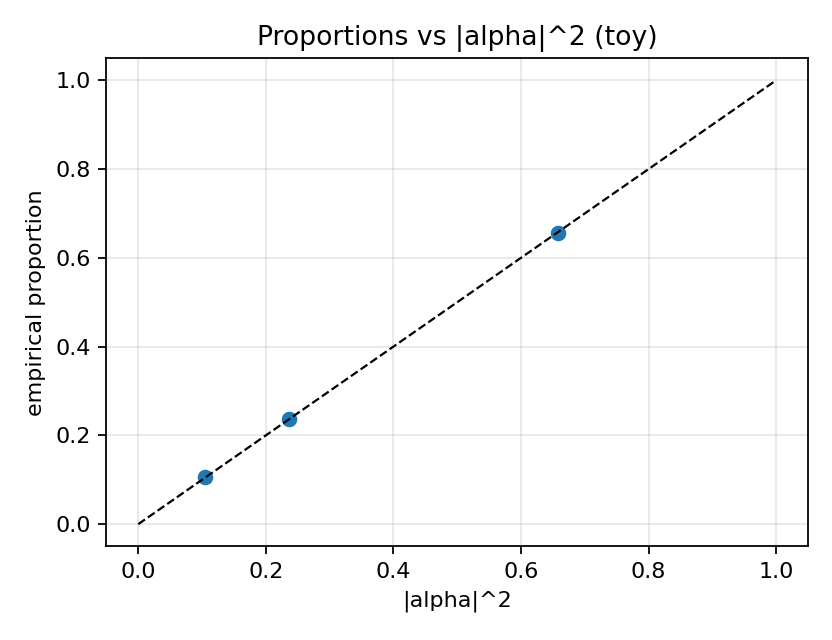
\includegraphics[width=0.72\linewidth]{../../artifacts/100.006/proportions_vs_amp2.png}\\
\emph{Figure 1.} Empirical sector proportions vs $|\alpha|^2$ (toy); points fall on the diagonal.
\end{center}

\begin{center}
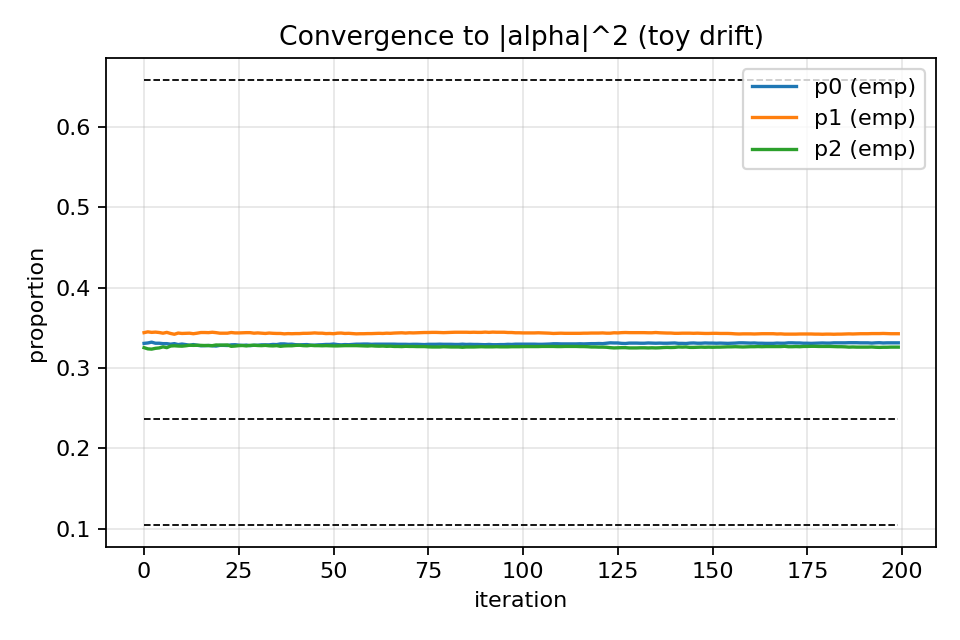
\includegraphics[width=0.72\linewidth]{../../artifacts/100.006/equilibrium_convergence.png}\\
\emph{Figure 2.} Convergence of empirical proportions to $|\alpha|^2$ with iterations (toy drift dynamics).
\end{center}

\section*{5. Tests and limits}
\textbf{Predictions.} (T1) Frequentist frequencies in repeated weak--then--strong protocols approach $|\alpha|^2$; (T2) small, transient pre--collapse biases follow the same scaling.\newline
\textbf{Limits.} If microstate ensembles fail to converge or show stable deviations, the drift model is falsified; energy accounting and no--signaling constraints apply as in 100.005.

\paragraph{Context.} Deterministic Born--rule accounts exist in the literature (e.g. Bohm--Valentini quantum equilibrium and Zurek's envariance arguments). FRC differs by deriving the weights from a resonance phase--locking picture with a small coherence drift and an explicit stationary measure \eqref{eq:rhostar}; the predictions above provide concrete discrimination against purely stochastic decoherence fits.

\section*{Reproducibility}
\section*{Methods checklist (for labs)}
\small\begin{itemize}
\item Platform and temperature (optomech/SC qubit; fridge stage).\n\item Readout channel (homodyne/di"ode IQ), sampling rate, integration window.\n\item Coherence proxy definition and calibration.\n\item Pre-collapse analysis: report Δln C and locking thresholds.\n\item Energy/entropy estimate: ΔQ≈k_B T ΔS from Δln C with error bars.\n\item Nulls/controls: off-critical runs; SSE/Lindblad fits without drift.\n\item Data/code release and seeds to regenerate figures.\n\end{itemize}
Run \verb|python code/100.006/make_figures.py|; figures are written to \verb|artifacts/100.006/|.

\section*{References}
\small
\begin{itemize}
  \item FRC~100.003 — Resonant Collapse (concept). DOI: \href{https://doi.org/10.5281/zenodo.15079820}{10.5281/zenodo.15079820}.
  \item FRC~100.004 — Quantum Foundations. DOI: \href{https://doi.org/10.5281/zenodo.17438174}{10.5281/zenodo.17438174}.
  \item FRC~100.005 — Thermodynamic Consistency. DOI: \href{https://doi.org/10.5281/zenodo.17438231}{10.5281/zenodo.17438231}.
  \item FRC~566.001 — Reciprocity \& UCC. DOI: \href{https://doi.org/10.5281/zenodo.17437759}{10.5281/zenodo.17437759}.
\end{itemize}

\section*{Appendix A: Sector weight sketch}
Let phases near sector $j$ be written as $\phi=\phi_j+\delta$ with a small deviation $\delta$. For the choice \eqref{eq:Cdef} one has
\( \ln C \approx \ln\big(|\alpha_j|^2\big) + \beta\cos\delta \), so the stationary density from \eqref{eq:rhostar} reads
\( \rho_\star(\delta) \propto |\alpha_j|^{2/k_*} e^{(\beta/k_*)\cos\delta} \).
Normalizing over $\delta$ gives a sector weight proportional to $|\alpha_j|^{2/k_*}$ times a factor that does not depend on $j$ (the Bessel function $I_0$). With the informational convention $k_*=1$ this yields $p_j\propto |\alpha_j|^2$. The same scaling holds for a broad class of $C$ whose local expansion near $\phi_j$ is quadratic in $\delta$; the Jacobian from the change of variables $\phi\mapsto (j,\delta)$ is sector--independent to leading order, so the $|\alpha|^2$ weight survives.

\end{document}
